%----------------------------------------------%
%---------------- INTRODUCCIÓN ----------------%
%----------------------------------------------%

\framecard{PROBLEM ANALYSIS}

\begin{frame}{Problem Analysis}{Main Objectives}
	\begin{columns}

		\begin{column}{0.5\textwidth}
			\centering \textsc{\Large Mathematics}
			\vspace{1mm}
			\hrule
			\vspace{3mm}
			
			\onslide<2->{To understand the movement of photons in relativistic spacetimes.}
		\end{column}

		\begin{column}{0.5\textwidth}
			\centering \textsc{\Large Computer Science}
			\vspace{1mm}
			\hrule
			\vspace{3mm}
			
			\onslide<3->{To design, implement and analyse the results of a relativistic raytracer.}
		\end{column}
	\end{columns}
\end{frame}

\framecard{BASIC MATHEMATICS}

\begin{frame}{Basic Mathematical Concepts}
	\large
	\begin{fullpageitemize}
		\item Lorentzian vector spaces.
		\pause
		\item Tensor algebra.
		\pause
		\item Differential (semi-Riemannian) geometry.
	\end{fullpageitemize}
\end{frame}

\begin{frame}{Basic Mathematical Concepts}{Lorentzian Vector Spaces}	
	A Lorentzian product $g$ in $V$ is a symmetric, non-degenerate, index 1 bilinear form in $V$.
	\pause
	\[
		v \in (V,g) \textrm{ is said to be } \pause\begin{cases}
			\textrm{spacelike} &\textrm{if } $g(v,v) > 0,\, v = 0$\\
			\pause
			\textrm{timelike} &\textrm{if } $g(v,v) < 0$ \\
			\pause
			\textrm{lightlike} &\textrm{if } $g(v,v) = 0,\, v \neq 0$.
		\end{cases}
	\]
\end{frame}

\begin{frame}{Basic Mathematical Concepts}{Lorentzian Vector Spaces}
	\centering
	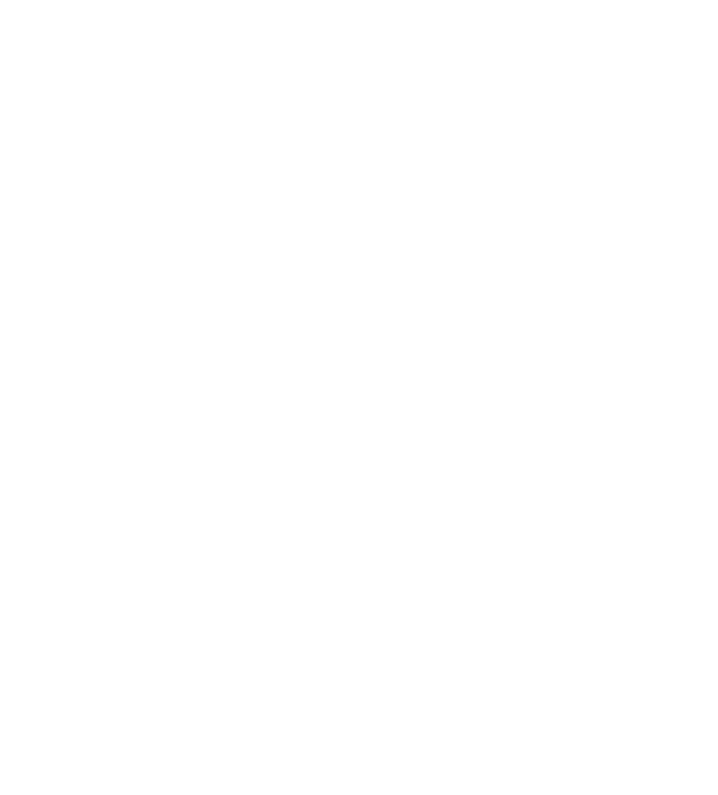
\includegraphics[height=0.7\paperheight]{gfx/timecones}
\end{frame}

\begin{frame}{Basic Mathematical Concepts}{Tensor Algebra}
	A \emph{tensor} $T$ of type $(r, s)$ in $V(K)$ is a multilinear map
	\[
		T \colon \underbrace{V^* \times \cdots \times V^*}_{\text{r copies}} \times \underbrace{V \times \cdots \times V}_{\text{s copies}} \longrightarrow K.
	\]
	
	\pause
	
	A basis of $\mathcal{T}_{(r,s)}(V)$ is
	\[
		\mathcal{B}_T = \{v_{i_1} \otimes \dots \otimes v_{i_r} \otimes \varphi^{j_1} \otimes \dots \otimes \varphi^{j_s}\},
	\]
	
	\pause
	where the coordinates are denoted by \[t^{i_1,\dots,i_r}_{j_1,\dots,j_s} = T(\varphi^{i_1}, \dots, \varphi^{i_r}, v_{j_1}, \dots, v_{j_s}).\]
\end{frame}

\begin{frame}{Basic Mathematical Concepts}{Differential Geometry}
	A \emph{smooth manifold} $M$ is a topological space that satisfies:
	\begin{itemize}
		\item $M$ is locally euclidean.
		\pause
		\item $M$ is Hausdorff.
		\pause
		\item $M$ has a countable topological basis.
	\end{itemize}
\end{frame}

\begin{frame}{Basic Mathematical Concepts}{Differential Geometry}
	\centering
	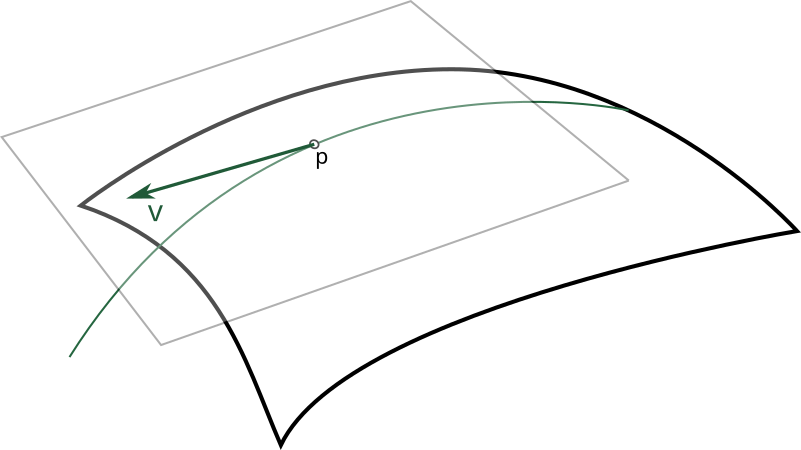
\includegraphics[height=0.4\paperwidth]{gfx/planotangente}
\end{frame}

\begin{frame}{Basic Mathematical Concepts}{Semi-Riemannian Geometry}
	\large
	\begin{fullpageitemize}
		\item Lorentzian metric: $g_p \colon T_pM\times T_pM \to \mathbb{R}$.
		\pause
		\item Lorentzian manifold: $(M,g)$.
		\pause
		\item Spacetime: a time oriented four dimensional $(M,g)$.
	\end{fullpageitemize}
\end{frame}

\framecard{$G = T$}

\framecard{$R_{\mu\nu} - \frac{1}{2}S g_{\mu\nu} = T_{\mu\nu}$}

\framecard{KERR SPACETIME}

\begin{frame}{Relativistic Spacetimes}{Kerr Metric}
	{\Large
		\begin{align*}
		ds^2 = &-dt^2 + \rho^2\left(\frac{dr^2}{\Delta} + d\vartheta^2\right) + \\
		&+ \left(r^2 + a^2\right)\textrm{\latolightfont sin}^2\vartheta d\varphi^2 + \\
		\nonumber
		&+ \frac{2r}{\rho^2}\left(a\textrm{\latolightfont sin}^2\vartheta d\varphi - dt\right).
		\end{align*}
	}
\end{frame}

\framepic{gfx/ergosfera}

%----------------------------------------------%
%----------------- GEODÉSICAS -----------------%
%----------------------------------------------%

\framecard{GEODESICS}

\begin{frame}{Geodesics}{Classic Equations}
	{\Huge
	\[
		\frac{d^2x^k}{dt^2} + \Gamma^k_{ij} \frac{d x^i}{dt} \frac{d x^j}{dt} = 0
	\]}
	\vfill
	\[
		\Gamma^m_{ij} = \frac{1}{2} g^{km} \left( \pd{}{x^i} g_{jk} + \pd{}{x^j} g_{ki} - \pd{}{x^k}g_{ij} \right)	
	\]
\end{frame}

\begin{frame}{Geodesics}{Classic Hamiltonian Approach}
	\large
	\begin{align*}
		\rho^2 \dot{t} &=-( aE\textrm{\latolightfont sin}^2\vartheta - L_z) + \frac{r^2+a^2}{\Delta}P, \\
		\rho^2 \dot{r} &= \sqrt{R}, \\
		\rho^2 \dot{\vartheta} &= \sqrt{\Theta}, \\
		\rho^2 \dot{\varphi} &=-( aE - \frac{L_z}{\textrm{\latolightfont sin}^2\vartheta}) + \frac{a}{\Delta}P.
	\end{align*}
\end{frame}

\begin{frame}{Geodesics}{Variational Formulation}
	\large
	\begin{align*}
		\dot{r} &= \frac{\Delta}{\rho^2} p_r, \quad \dot{\vartheta} = \frac{1}{\rho^2}p_\vartheta, \quad
		\dot{\varphi} = \pd{}{p_\varphi}\left( \frac{R + \Delta\Theta}{2\Delta\rho^2} \right), \\
		\dot{p}_r &= - \pd{}{r} \left( - \frac{\Delta}{2\rho^2}p_r^2 - \frac{1}{2\rho^2}p_\vartheta^2 + \left( \frac{R + \Delta\Theta}{2\Delta\rho^2} \right) \right), \\
		\dot{p}_\vartheta &= - \pd{}{\vartheta} \left( - \frac{\Delta}{2\rho^2}p_r^2 - \frac{1}{2\rho^2}p_\vartheta^2 + \left( \frac{R + \Delta\Theta}{2\Delta\rho^2} \right) \right).
	\end{align*}
	
\end{frame}


%----------------------------------------------%
%------------------- SET UP -------------------%
%----------------------------------------------%

\framecard{SET UP}

{\setbeamercolor{background canvas}{bg=white}
	\begin{frame}[plain]{Set Up}
		\centering
		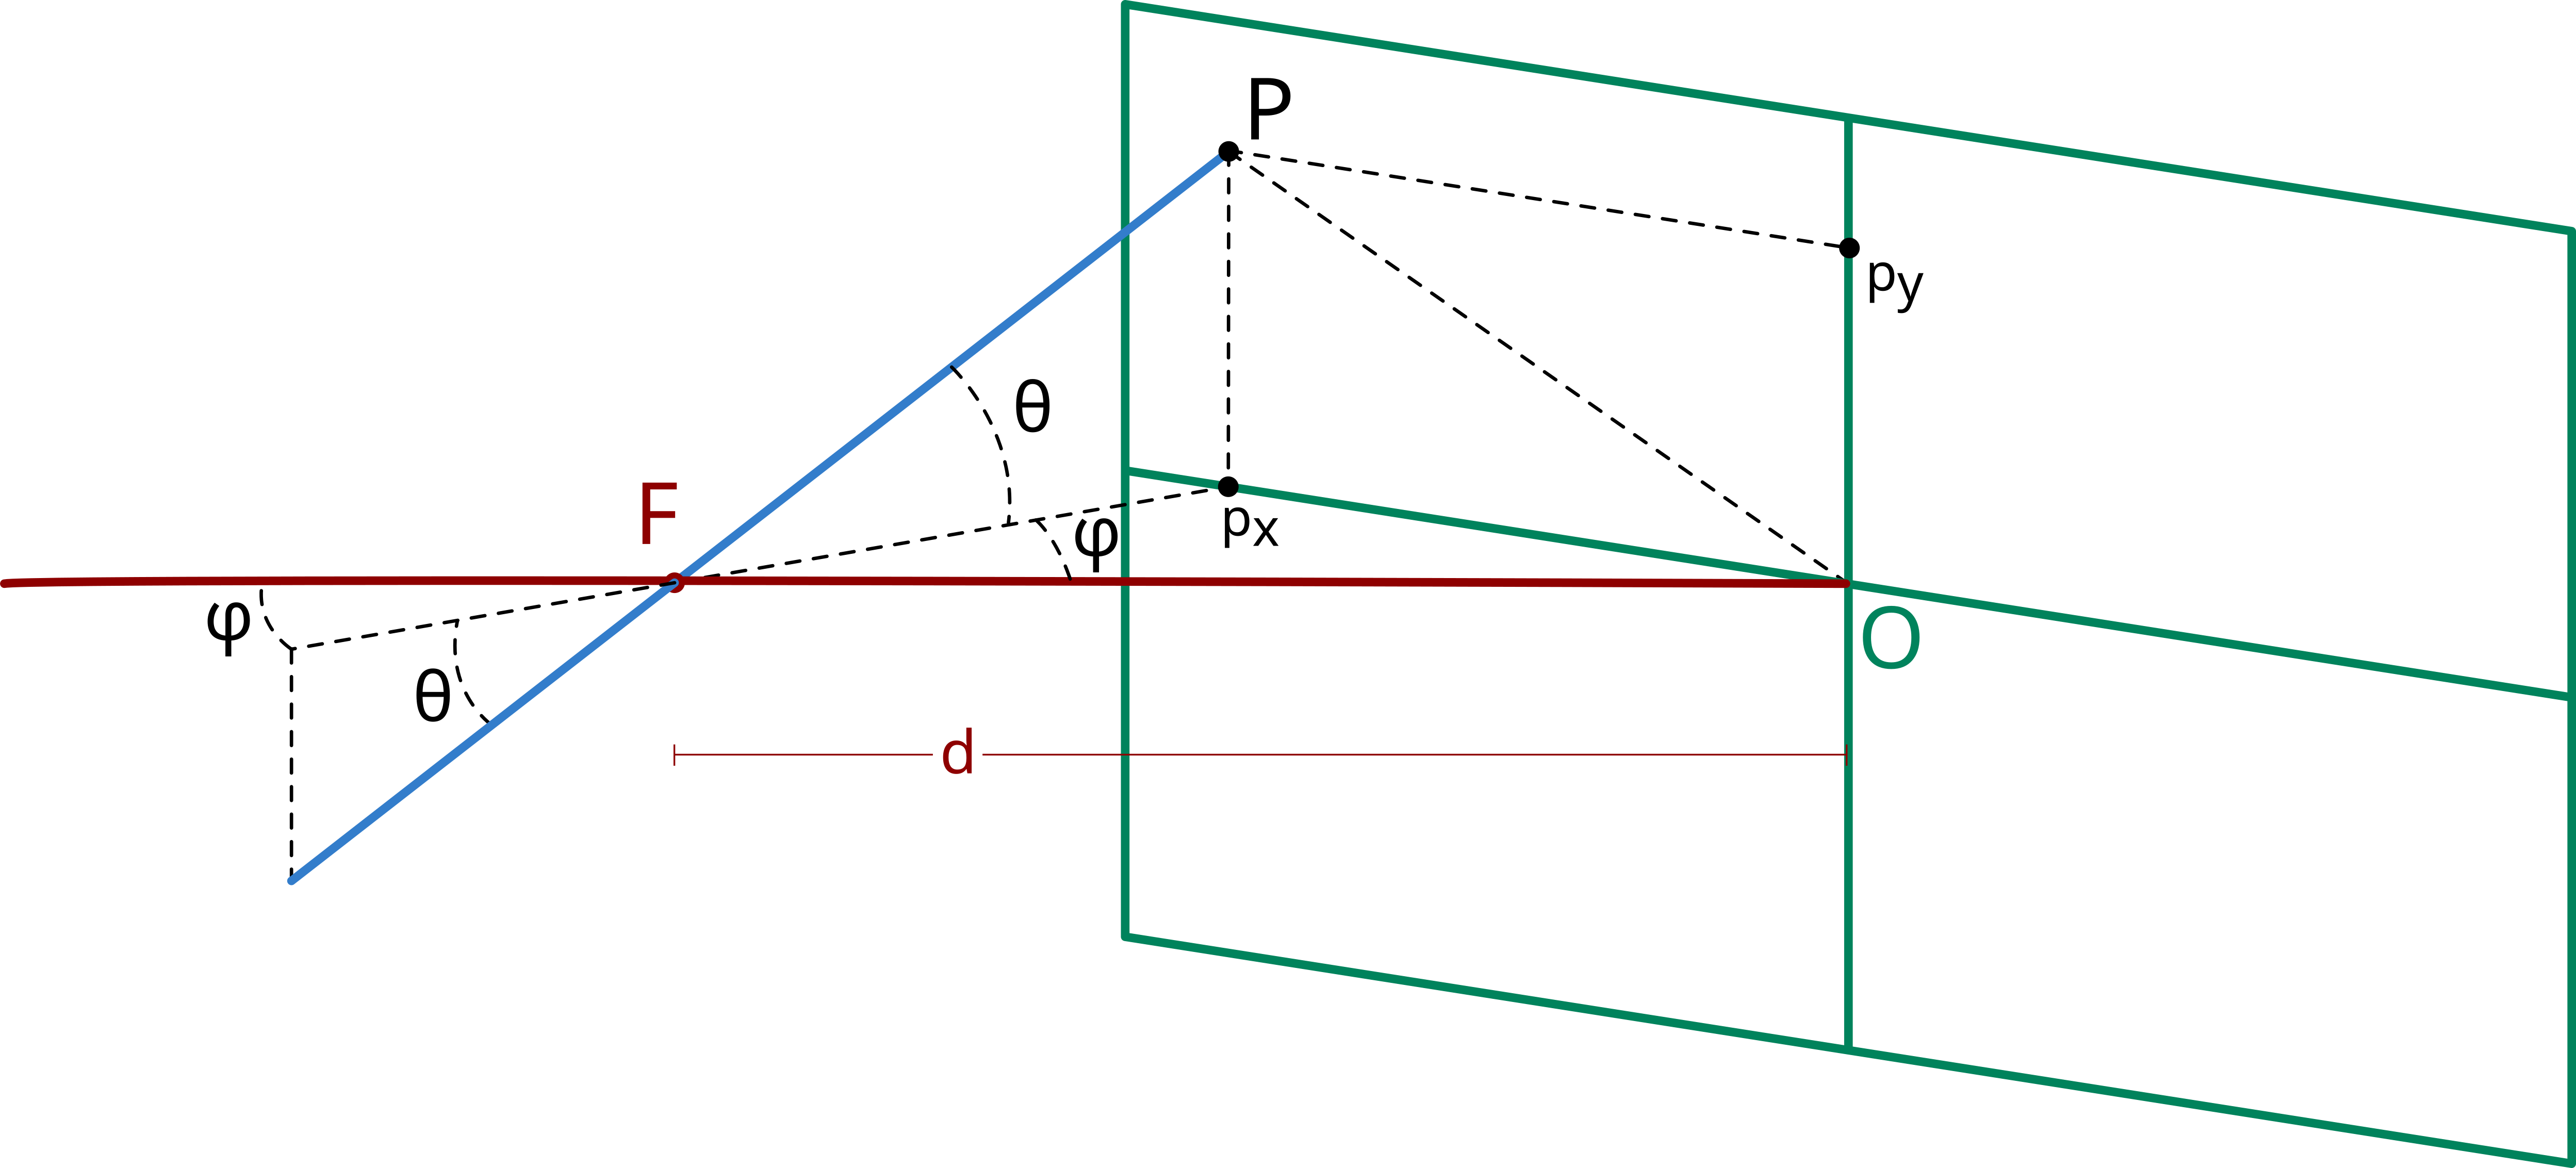
\includegraphics[width=0.8\paperwidth]{gfx/pinhole}
	\end{frame}
}

%\frameanimation{gfx/blech-}{1}{90}{20}

%----------------------------------------------%
%------------------- INFORM -------------------%
%----------------------------------------------%

\framecard{SOFTWARE}

\begin{frame}{Software}{Basic Algorithm}
	{
	\tiny
	\begin{algorithm}[H]
		%\caption{High-level abstraction of the ray tracer}
		\begin{algorithmic}[1]
			\Function{Ray Tracer}{}
			\State ODEsystem $\gets$ Kerr spacetime geodesics ODE
			\State Camera $\gets$ Pinhole camera model
			\State Geodesics $\gets \{\emptyset\}$
			\For{pixel $p = (p_x, p_y)$ in the Camera sensor}
			\State initCond $\gets$ initConditions($p_x$, $p_y$)
			\State $\gamma_{xy} \gets$ solveIVP(ODEsystem, initCond)
			\State Geodesics $\gets$ Geodesics $\cup$ $\gamma_{xy}$
			\EndFor
			\Return{Geodesics}
			\EndFunction
		\end{algorithmic}
	\end{algorithm}
	}
\end{frame}

\begin{frame}{Software}{Runge-Kutta}
	\[
	\Large
	\begin{split}
		\dot{y} &= f(t,y) \\
		y(t_0) &= y_0
	\end{split}
	\rightarrow
	\begin{cases}
		y_{n+1} &= y_n + h \sum\limits_{i=1}^s b_i k_i\\
		y^*_{n+1} &= y_n + h \sum\limits_{i=1}^s b^*_i k_i,
	\end{cases}
	\]
	\vspace{2mm}
	\[
		k_i = f(t_n + c_ih, y_n + h\sum_{j=1}^{i-1} a_{ij} k_j).
	\]
\end{frame}

\begin{frame}{Software}{Runge-Kutta Step}
	\centering
	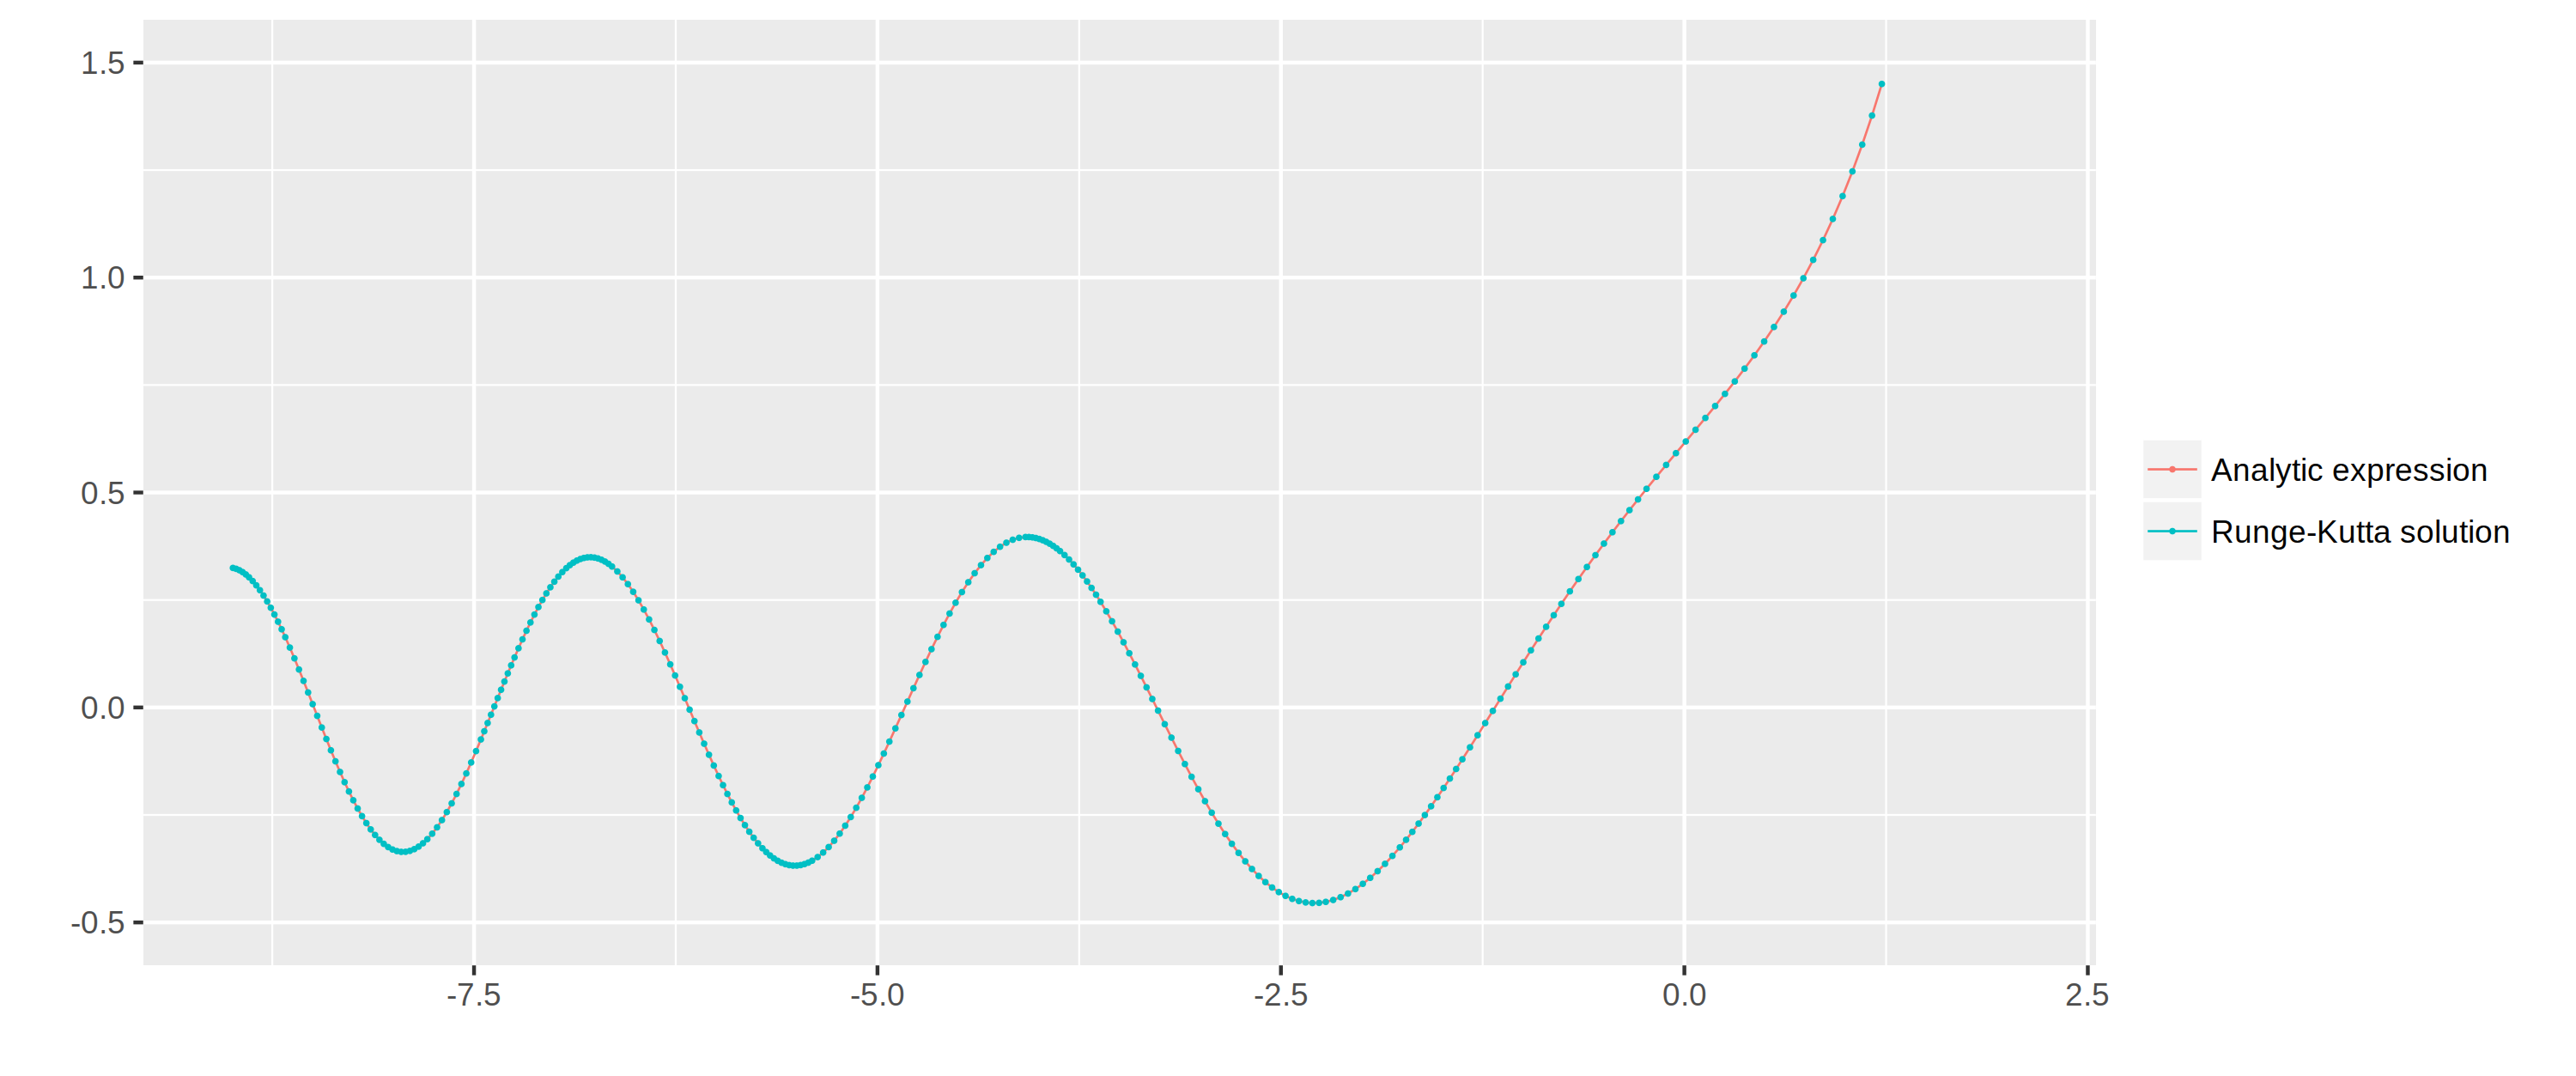
\includegraphics[width=0.8\paperwidth]{gfx/analytic}
\end{frame}

\begin{frame}{Software}{Basic Algorithm}
{
	\tiny
	\begin{algorithm}[H]
		%\caption{High-level abstraction of the ray tracer}
		\begin{algorithmic}[1]
			\Function{Ray Tracer}{}
			\State ODEsystem $\gets$ Kerr spacetime geodesics ODE
			\State Camera $\gets$ Pinhole camera model
			\State Geodesics $\gets \{\emptyset\}$
			\For{pixel $p = (p_x, p_y)$ in the Camera sensor}
			\State initCond $\gets$ initConditions($p_x$, $p_y$)
			\State $\gamma_{xy} \gets$ solveIVP(ODEsystem, initCond)
			\State Geodesics $\gets$ Geodesics $\cup$ $\gamma_{xy}$
			\EndFor
			\Return{Geodesics}
			\EndFunction
		\end{algorithmic}
	\end{algorithm}
}
\end{frame}

\begin{frame}{Software}{GPU Architecture}
	\centering
	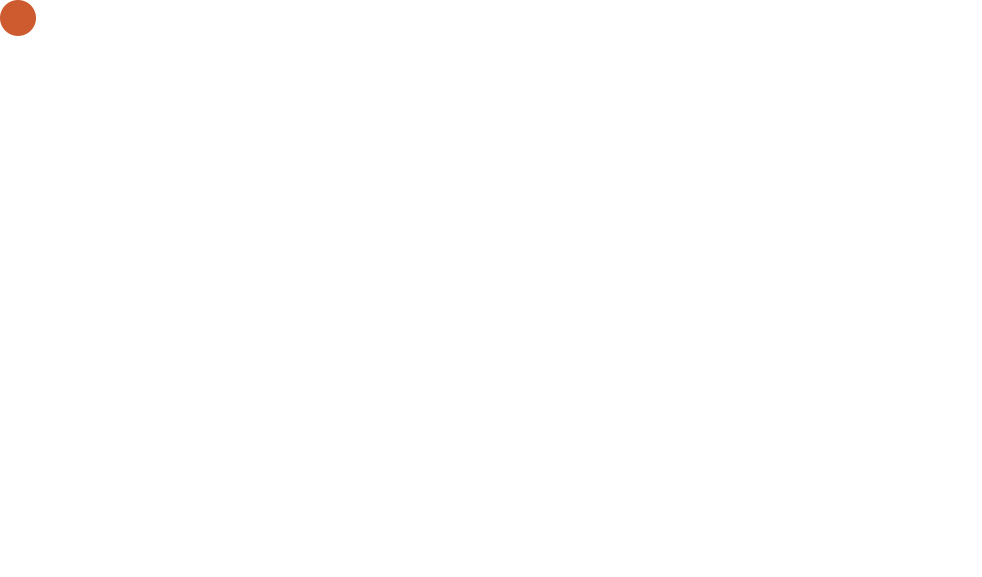
\includegraphics[width=0.6\paperwidth]{gfx/cores01}
\end{frame}

\begin{frame}{Software}{GPU Architecture}
\centering
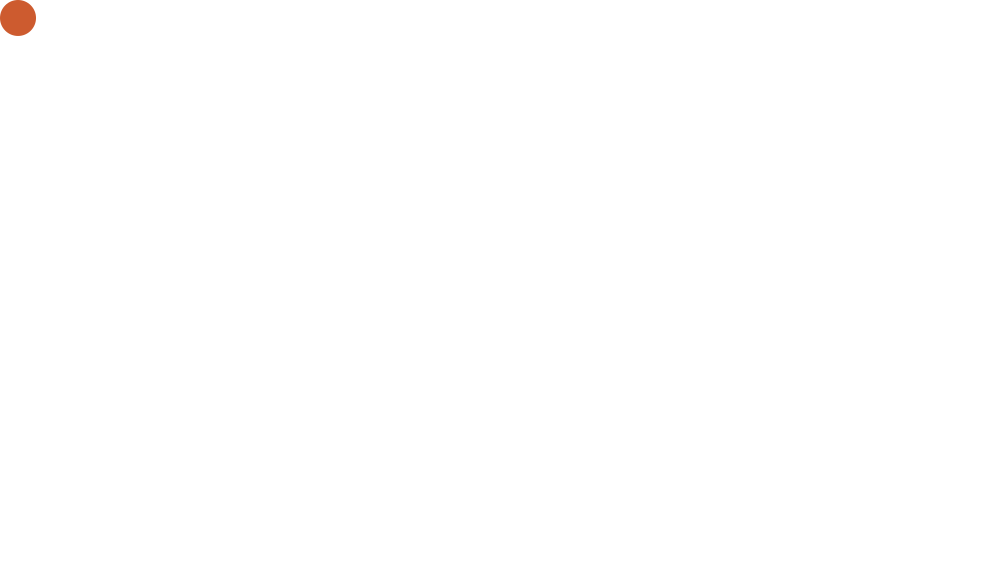
\includegraphics[width=0.6\paperwidth]{gfx/cores02}
\end{frame}

\begin{frame}{Software}{GPU Architecture}
	\centering
	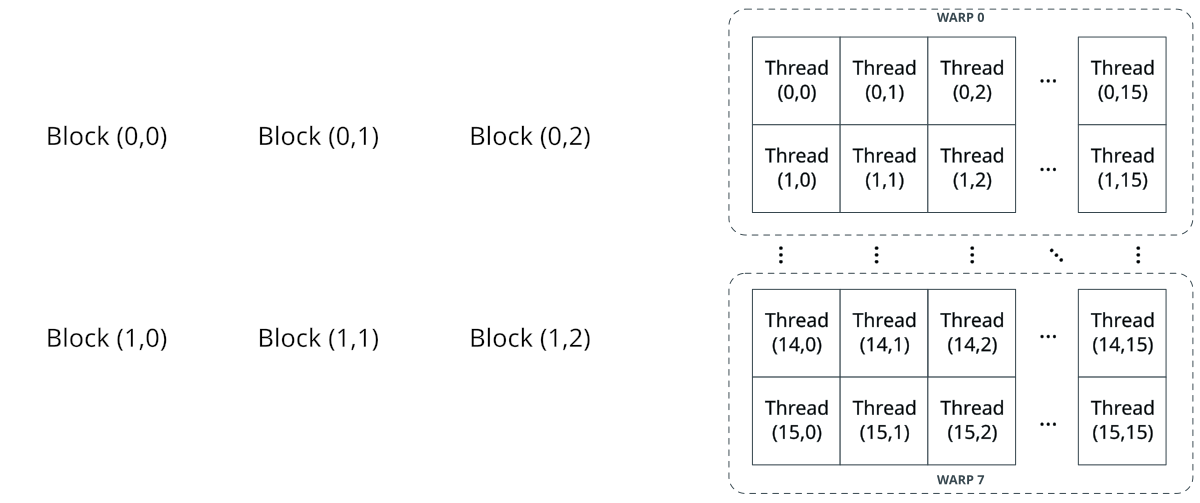
\includegraphics[width=0.9\paperwidth]{gfx/cudagrid}
\end{frame}

\begin{frame}{Software}{GPU Architecture}
\centering
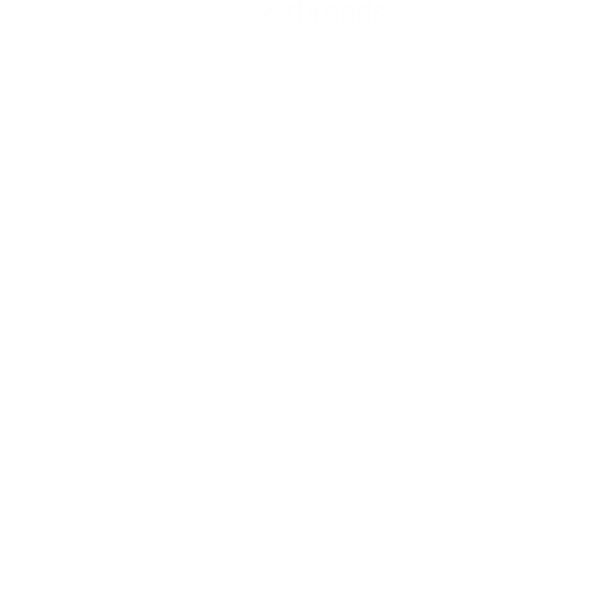
\includegraphics[height=0.7\paperheight]{gfx/owncudagrid}
\end{frame}

%----------------------------------------------%
%------------------ RESULTS -------------------%
%----------------------------------------------%

\framecard{TECHNICAL RESULTS}

\begin{frame}{Technical Results}{Runge-Kutta Step}
	\centering
	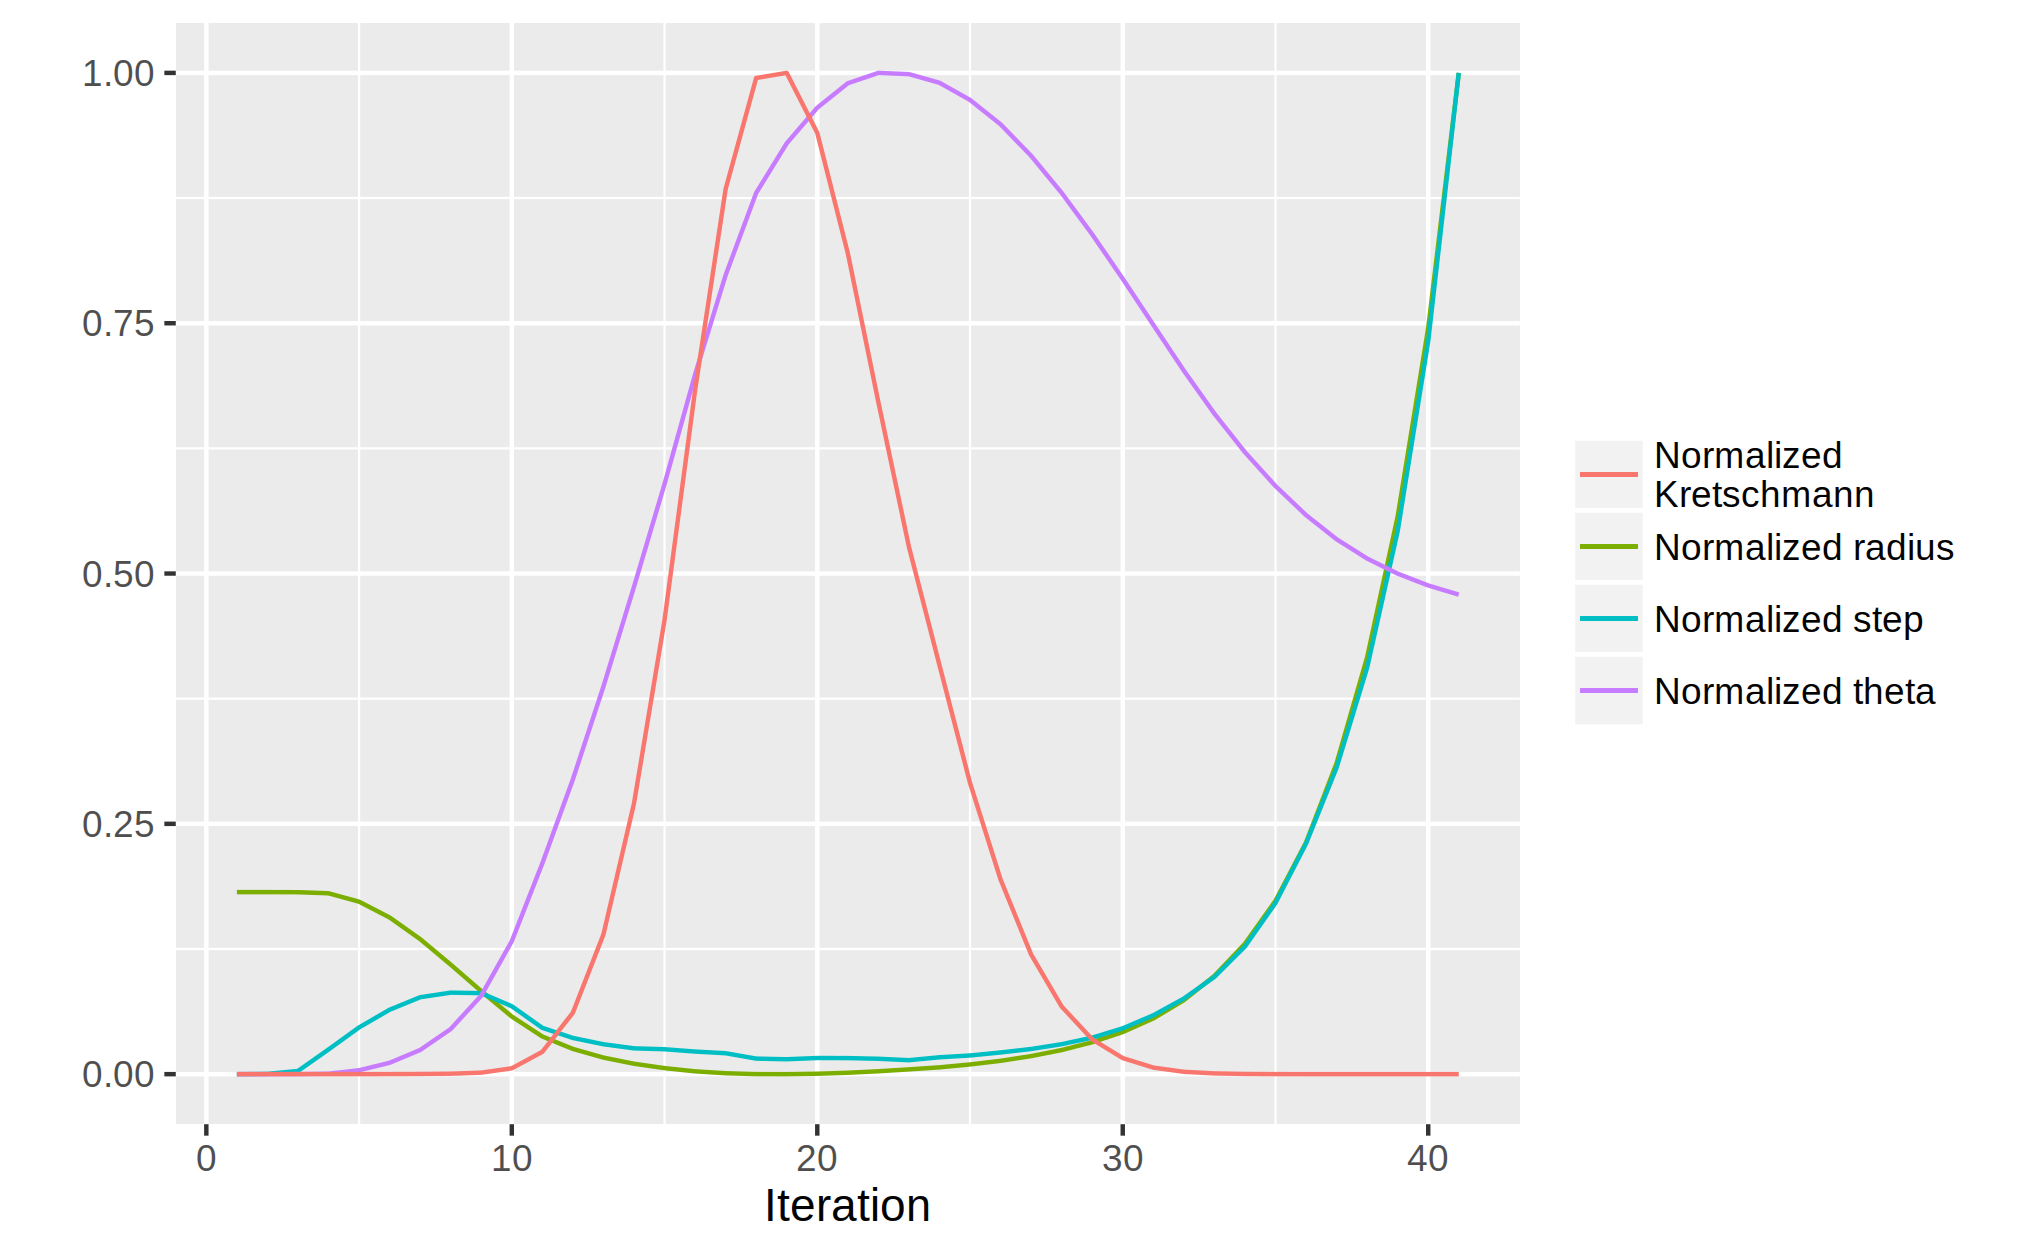
\includegraphics[width=0.7\paperwidth]{gfx/kretschmann}
\end{frame}

\begin{frame}{Technical Results}{Speed Up}
\centering
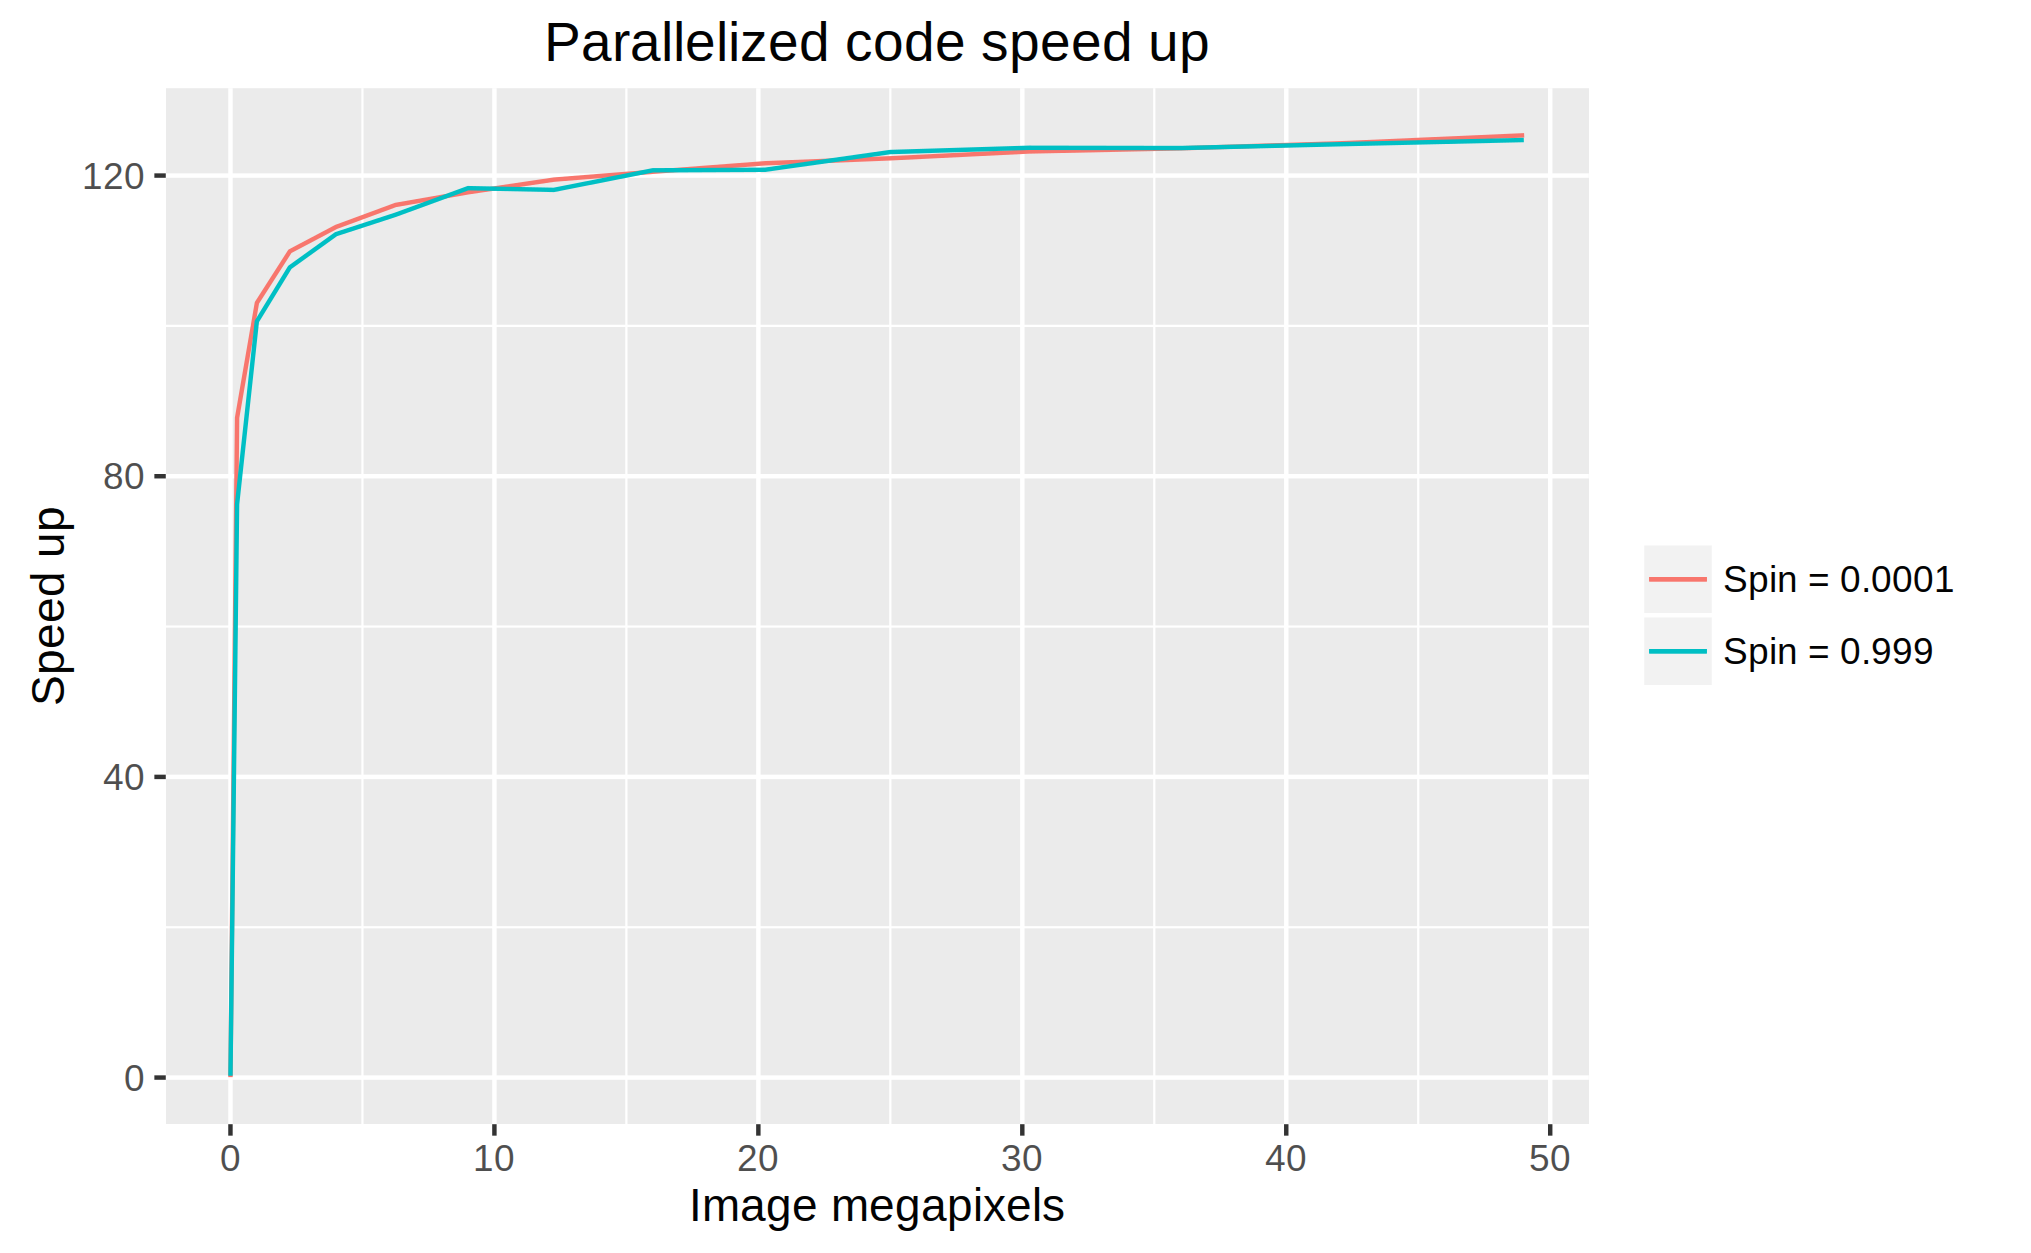
\includegraphics[width=0.7\paperwidth]{gfx/speedup}
\end{frame}

\framecard{RELATIVISTIC ABERRATION}

\frameanimation{gfx/blech-}{1}{90}{20}

\framecard{IMAGE CONSTRUCTION}

\framepic{gfx/complete00}

\framepic{gfx/complete01}

\framepic{gfx/complete02}

\framepic{gfx/complete03}

\framepic{gfx/complete04}

\framecard{EUCLIDEAN CASE}

\framepic{gfx/euclidean01}

\framepic{gfx/euclidean02}

\framecard{3D REPRESENTATION}

\framepic{gfx/3D_01}

\framepic{gfx/3D_02}

\framepic{gfx/3D_03}

\framecard{SPIN}

\frameanimation{gfx/spin}{1}{50}{15}

\framecard{SHADOW}

\frameanimation{gfx/patchedShadow}{1}{63}{20}

\frameanimation{gfx/patchedShadowVertical}{1}{61}{20}

\framecard{ANIMATIONS}

\frameanimation{gfx/cinema01_}{1}{126}{20}

\frameanimation{gfx/cinema02_}{1}{63}{12}

\framecard{CONCLUSIONS}


%-----------------------------

%\frameanimation{../../Software/Examples/anim_01_cinematographic}{1}{126}{20}
%\frameanimation{../../Software/Examples/anim_04_cinematographic}{1}{32}{13}

%\begin{frame}[plain]
%	\movie[width=
%	\paperwidth,borderwidth=10pt,poster,showcontrols]{\includegraphics[width=\paperwidth]{../../Software/Examples/anim_01_cinematographic001}}{out.avi}
%\end{frame}


%\begin{frame}
%	\begin{center}
%		\movie[width=\textwidth,showcontrols=true]
%		{\includegraphics[width=\textwidth]{../../Software/Examples/anim_01_cinematographic001}}{out.avi}
%	\end{center}
%\end{frame}

%\begin{frame}{sqf}
%	
%	\includemedia[
%	width=0.6\linewidth,height=0.6\linewidth,
%	activate=pageopen,
%	transparent,
%	addresource=prueba.mp4,
%	flashvars={
%		source=prueba.mp4     % same path as in addresource!
%		&loop=true           % loop video
%		&scaleMode=letterbox % preserve aspect ratio
%	}
%	]{}{VPlayer9.swf}
%\end{frame}

%\begin{frame}[plain]
%	
%	\includemedia[
%	width=0.6\linewidth,height=0.6\linewidth,
%	activate=pageopen,
%	transparent,
%	addresource=out.avi,
%	flashvars={
%		source=out.avi     % same path as in addresource!
%		&loop=true           % loop video
%		&scaleMode=letterbox % preserve aspect ratio
%	}
%	]{}{VPlayer9.swf}
%\end{frame}

%\begin{frame}[plain]
%	\movie[width=
%	\paperwidth,borderwidth=10pt,poster,showcontrols]{\includegraphics[width=\paperwidth]{../../Software/Examples/anim_01_cinematographic001}}{../../Software/Examples/out.mp4}
%\end{frame}

%{
%	\usebackgroundtemplate{%
%		\setbeamercolor{background canvas}{bg=black}
%		\tikz[overlay,remember picture] \node[opacity=1, at=(current page.center)] {
%			\movie[width=1.6cm,height=9cm,loop,poster,autostart]{}{../../Software/Examples/out.mov}
%		};
%	}
%	\begin{frame}[plain]
%	\end{frame}
%}